%\chapter*{Appendix A: Publications}
\chapter{Publications}
%\addchaptertocentry{Appendices}
%\thispagestyle{appdx}

\textbf{Shruthi Mohan}, Teena Koshy, Perumal Vekatachalam, Sheela Nampoothiri,
Dhanya Yesodharan, Kalpana Gowrishankar, Jeevan Kumar, Latha Ravichandran,
Santhosh \linebreak Joseph, Anupama Chandrasekaran, Solomon FD Paul.
Subtelomeric rearrangements in Indian children with idiopathic intellectual
disability/developmental delay: frequency estimation and clinical correlation
using FISH. \textit{In press: \textbf{Indian Journal of Medical Research}}

\textbf{Shruthi Mohan}, Vettriselvi Venkatesan, Teena Koshy, Solomon FD Paul,
Perumal Venkatachalam. Genomic imbalances in subjects with idiopathic
intellectual disability detected by multiplex ligation-dependent probe
amplification. \textit{In press: \textbf{Journal of Genetics}}

\textbf{Shruthi Mohan}, Sheela Nampoothiri, Dhanya Yesodharan, Vettriselvi
Venkatesan,\linebreak Teena Koshy, Solomon FD Paul, Perumal Venkatachalam.
Reciprocal microduplication  of the Williams-Beuren syndrome (7q11.23) region.
\textit{Under review: \textbf{Lab Medicine}}

Teena Koshy, Vettriselvi Venkatesan, Kalpana Gowrishankar, Venkatachalam
Perumal, \textbf{Shruthi Mohan}, Solomon FD Paul. Mutation analysis of Tbx1 in
children with \linebreak conotruncal heart anomalies from a referral hospital in
South India. \textit{Under Review: \textbf{Indian Journal of Pediatrics}}

\cleardoublepage

\section*{Manuscript in press (Indian Journal of Medical Research)}

\begin{figure}[!h]

\includegraphics[width=\linewidth,height=\textheight,keepaspectratio]{Appendices/IJMRacceptance1.pdf}
\end{figure}


\begin{quoting}[indentfirst=false]
\textit{Abstract of IJMR\textunderscore 622\textunderscore 14}

\textit{Background}: Subtelomeres are prone to deleterious rearrangements owing to their
proximity to unique sequences on one end and telomeric repetitive sequences,
which increase their tendency to recombine, on the other. These subtelomeric
rearrangements resulting in segmental aneusomy are reported to contribute to the
aetiology of idiopathic intellectual disability/developmental delay (ID/DD) and
fluorescence in situ hybridization (FISH) is a sensitive and rapid method to
detect such rearrangements.

\textit{Methods}: One hundred and twenty seven subjects with idiopathic ID/DD were tested for subtelomeric rearrangements using karyotyping and FISH. Blood samples were cultured, harvested, fixed and GTG banded using standard protocols. FISH was performed using the manufacturer’s protocol with slight modifications.
Results: Rearrangements involving the subtelomeres were observed in 7.8\% of the
tested sample population. Detection of rearrangements visible at the resolution
of the karyotype constituted 2.3\%, while those rearrangements detected only
with FISH constituted 5.5\%. Five deletions and five unbalanced translocations
were detected. Analysis of parental samples wherever possible was informative
regarding the inheritance of the rearrangement.

\textit{Discussion}: Our study was retrospective, and in order to reduce selection bias,
we did not use a stringent inclusion criteria. The observed frequency is within
the reported range of 0–35\% and is representative of the Indian population,
from which data is very limited. All abnormal genotypes were clinically
correlated. Further analysis with array technologies present a future prospect.
Our results emphasize the need to test individuals with ID/DD for subtelomeric
rearrangements using sensitive and cost-effective methods such as FISH.
\end{quoting}

\cleardoublepage
\section*{Manuscript in press (Journal of Genetics)}

\begin{figure}[!h]
\includegraphics[width=\linewidth,height=\textheight,keepaspectratio]{Appendices/Jgenacceptance.pdf}
\end{figure}

\begin{figure}[!b]
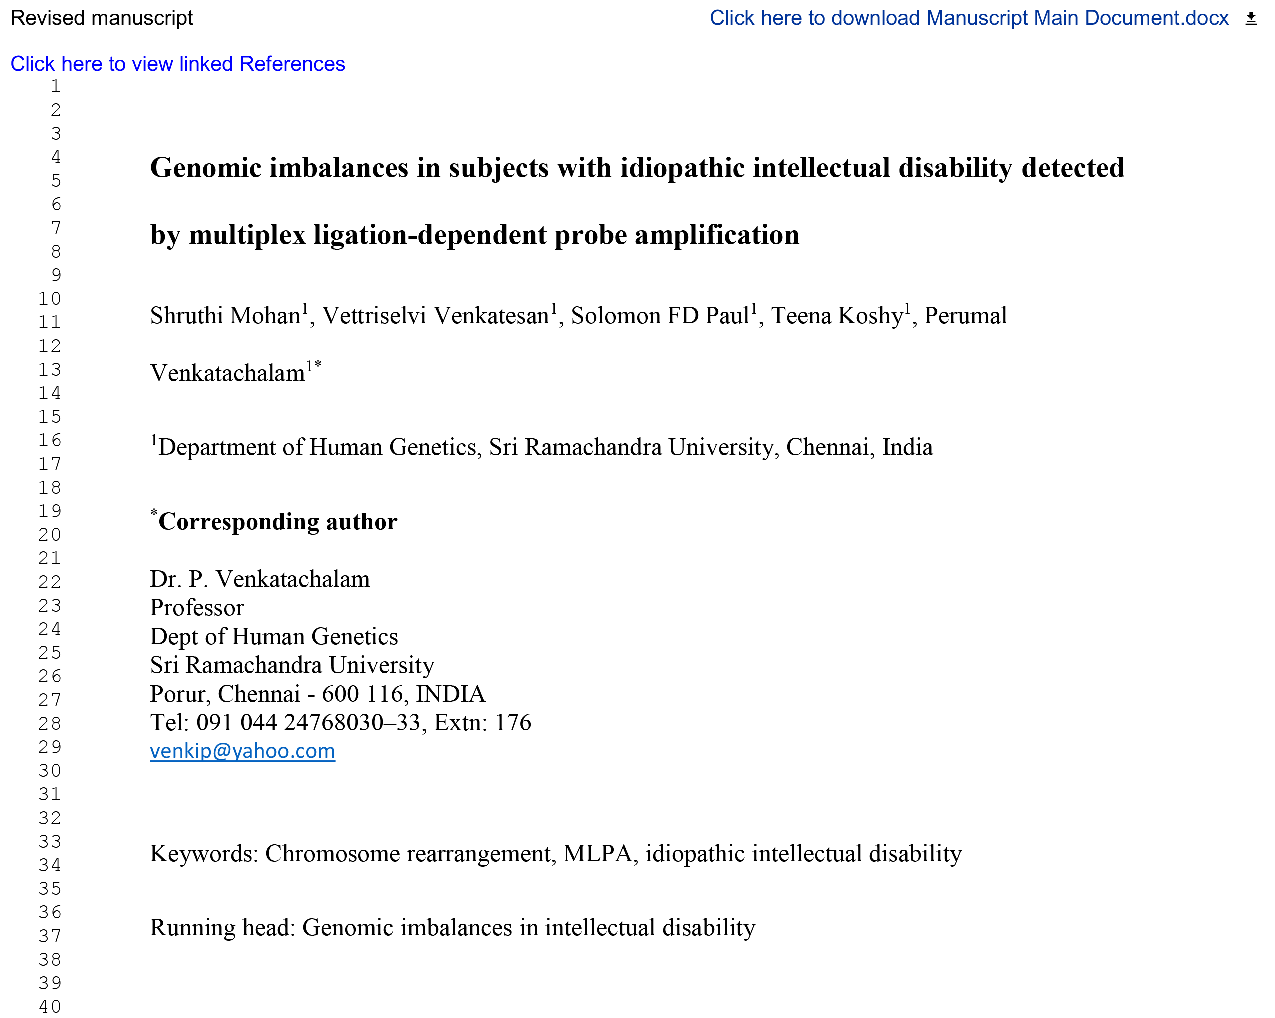
\includegraphics[keepaspectratio,scale=.6]{Appendices/Jgenarticle.pdf}
\end{figure}

\chapter{Presentations}

\textbf{Shruthi Mohan}, Teena Koshy, Solomon FD Paul, Latha Ravichandran, Venkatachalam P. Detection of subtelomeric rearrangements in idiopathic mental retardation by fluorescence in situ hybridization. 5th Annual Conference on Genetic and Molecular Diagnosis in Modern Medicine, SRM, Chennai; 2012.

\textbf{Shruthi Mohan}, Teena Koshy, Venkatachalam P, Solomon FD Paul, Latha Ravichandran, Kalpana Gowrishankar, Sheela Nampoothiri, Raheema Beevi, Suji Kumari. Subtelomeric rearrangements in children with idiopathic mental retardation. Next Revolution in Genetics and Genomics, Sir Gangaram Hospital, New Delhi; 2013.

\cleardoublepage

\chapter{Ethics Committee Approval}

\noindent%
\begin{minipage}{\linewidth}% to keep image and caption on one page
\makebox[\linewidth]{%        to center the image
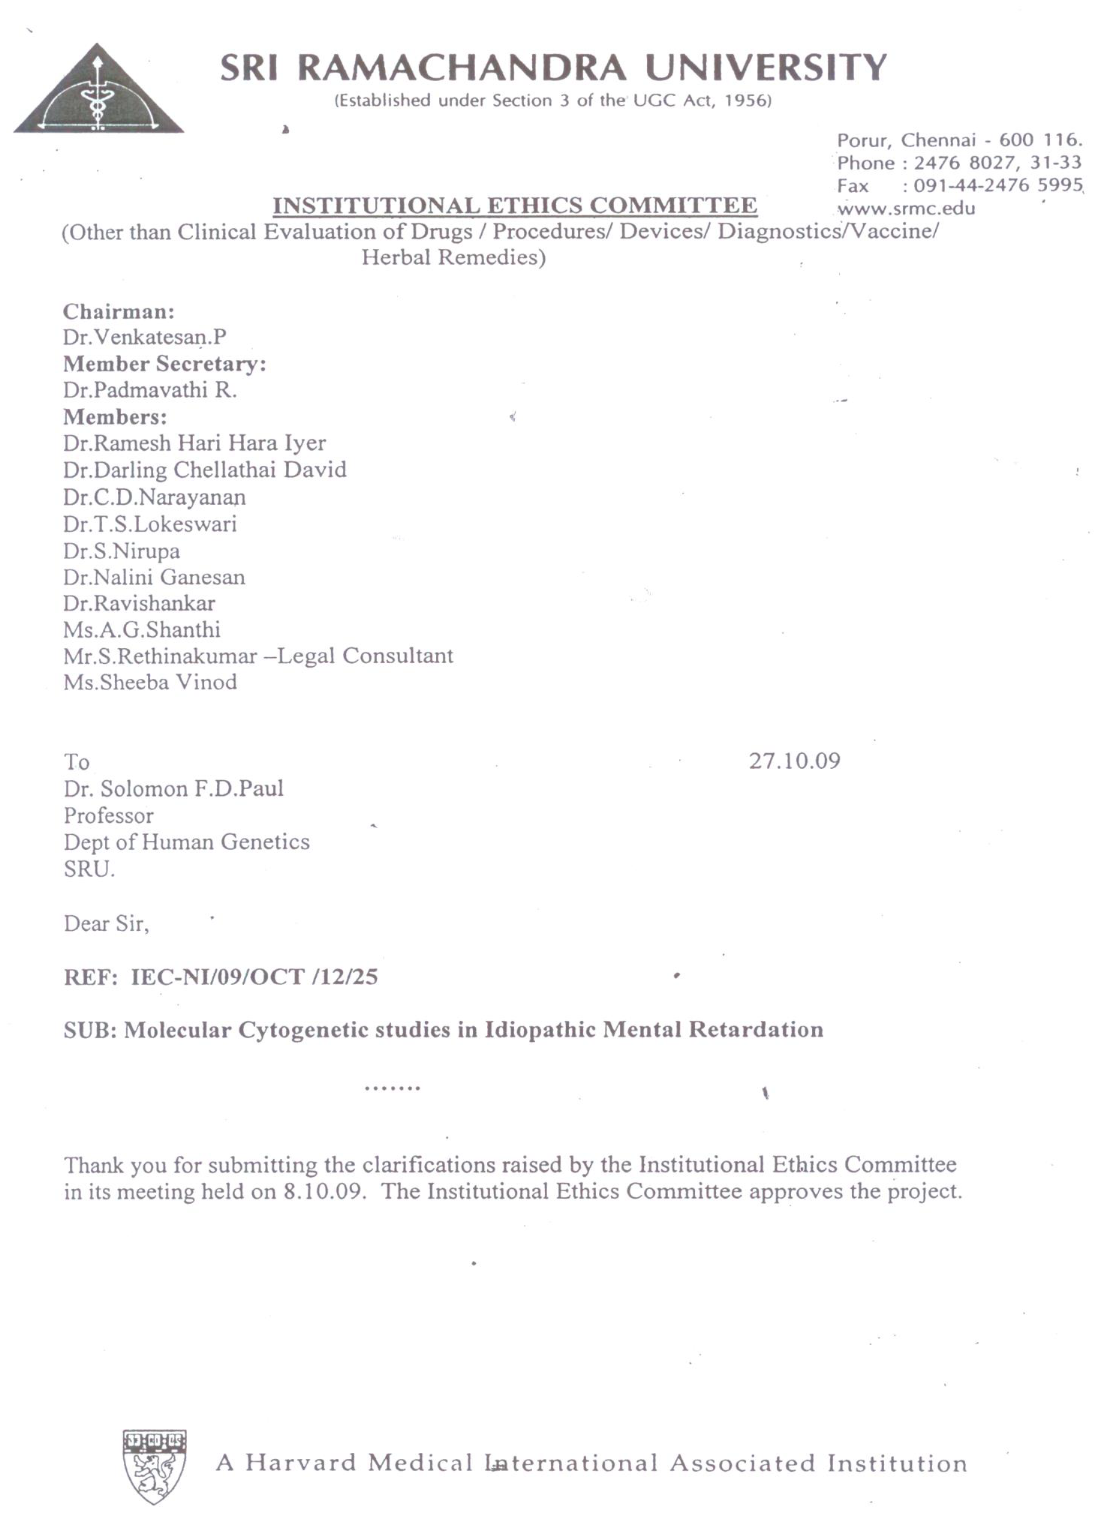
\includegraphics[width=\linewidth,height=\textheight,keepaspectratio]{Appendices/Appendix2.pdf}}
\end{minipage}

\noindent%
\begin{minipage}{\linewidth}% to keep image and caption on one page
\makebox[\linewidth]{%        to center the image
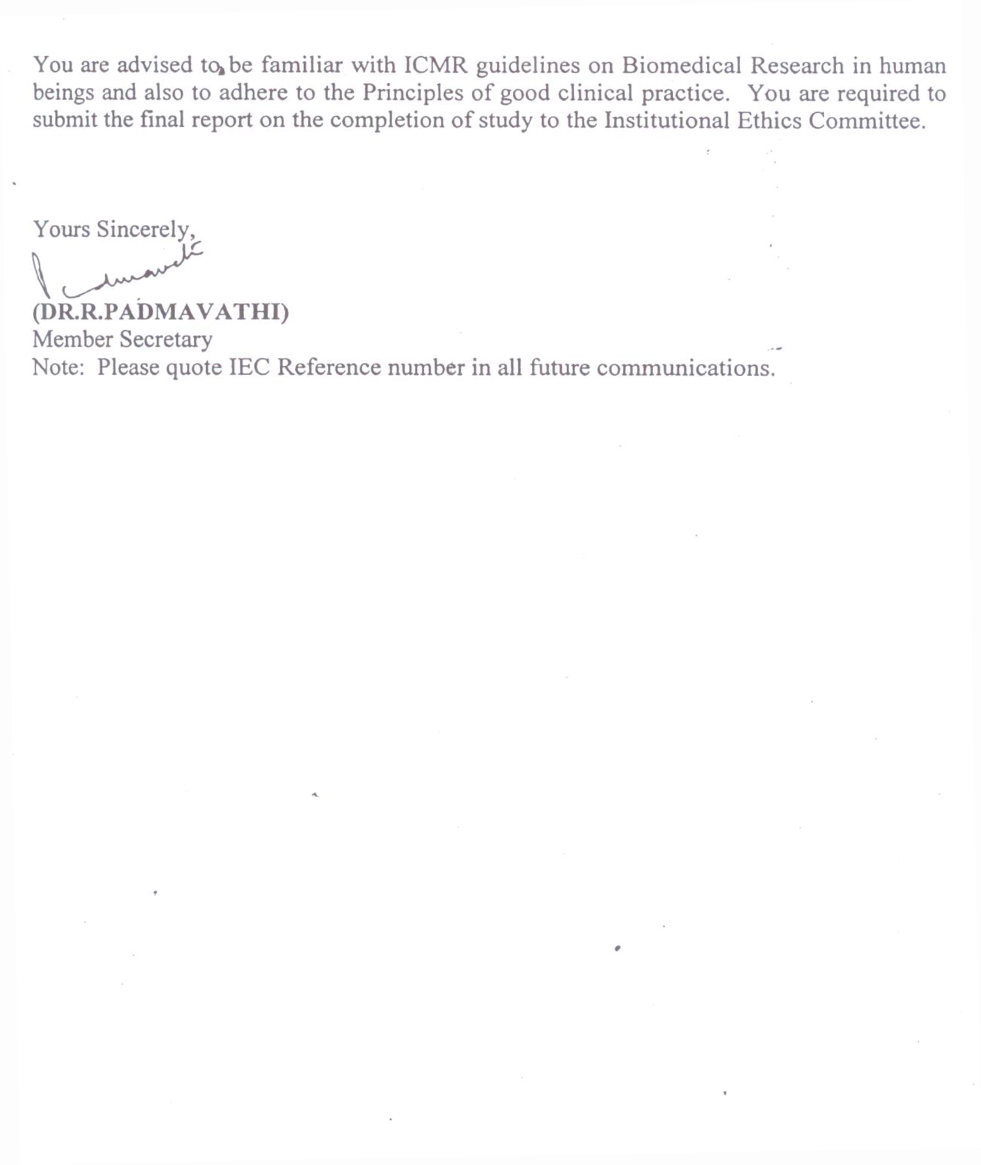
\includegraphics[width=\linewidth,height=\textheight,keepaspectratio]{Appendices/Appendixpg2.pdf}}
\end{minipage}


\chapter{Proforma and Informed Consent}

\noindent%
\begin{minipage}{\linewidth}% to keep image and caption on one page
\makebox[\linewidth]{%        to center the image
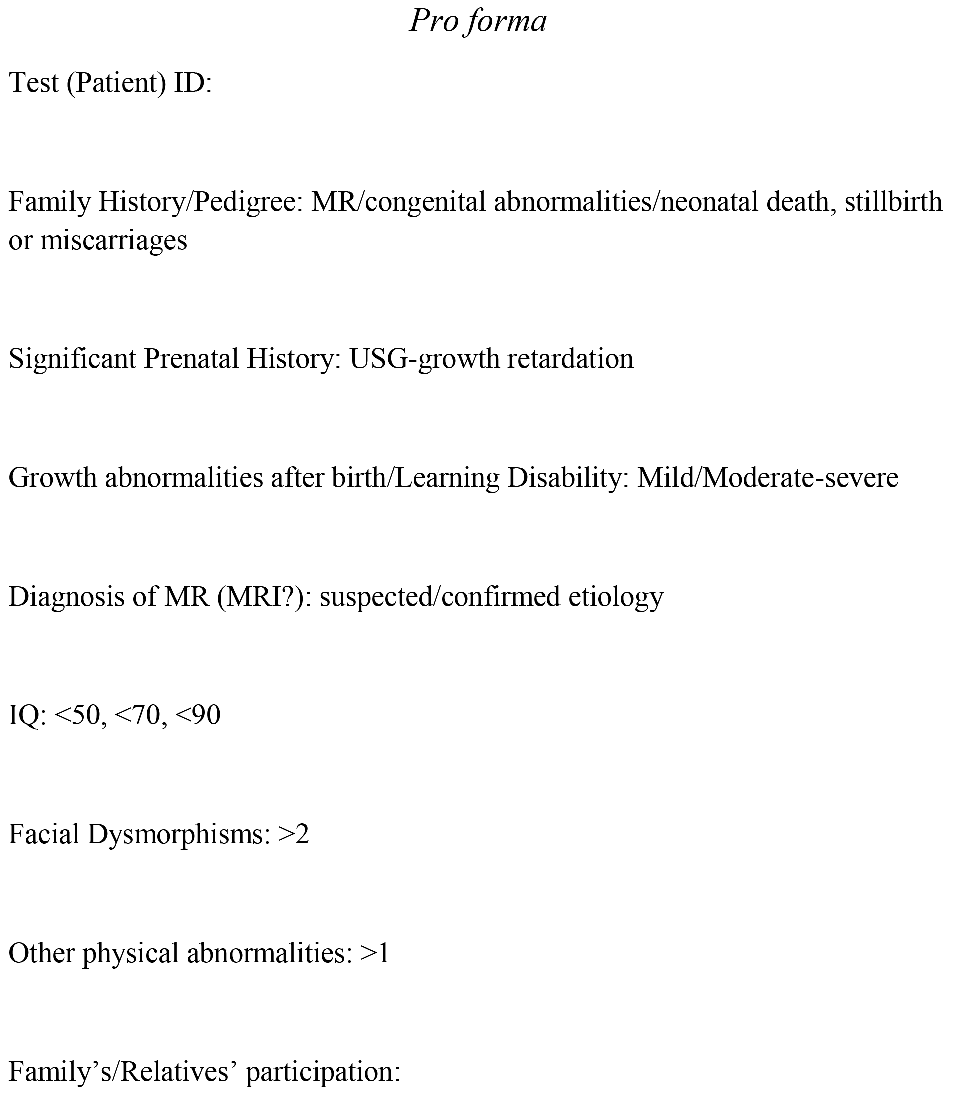
\includegraphics[width=\linewidth,height=\textheight,keepaspectratio]{Appendices/Appendix3a.pdf}}
\end{minipage}
\clearpage

\noindent%
\begin{minipage}{\linewidth}% to keep image and caption on one page
\makebox[\linewidth]{%        to center the image
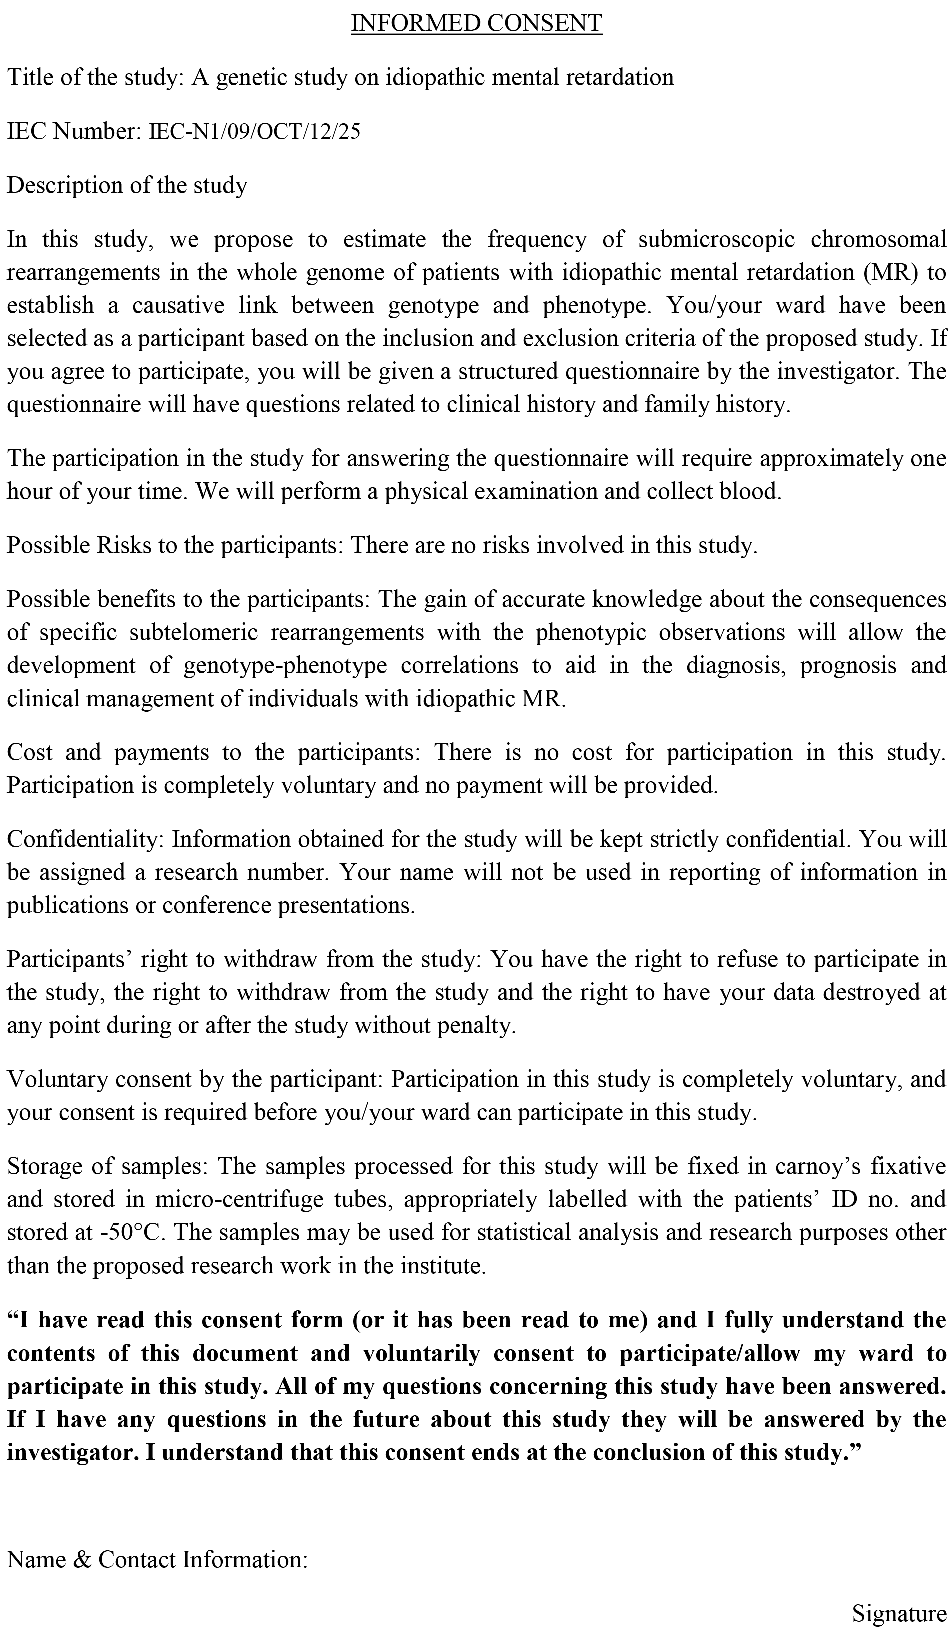
\includegraphics[width=\linewidth,height=\textheight,keepaspectratio]{Appendices/Appendix3b.pdf}}
\end{minipage}
\clearpage

\noindent%
\begin{minipage}{\linewidth}% to keep image and caption on one page
\makebox[\linewidth]{%        to center the image
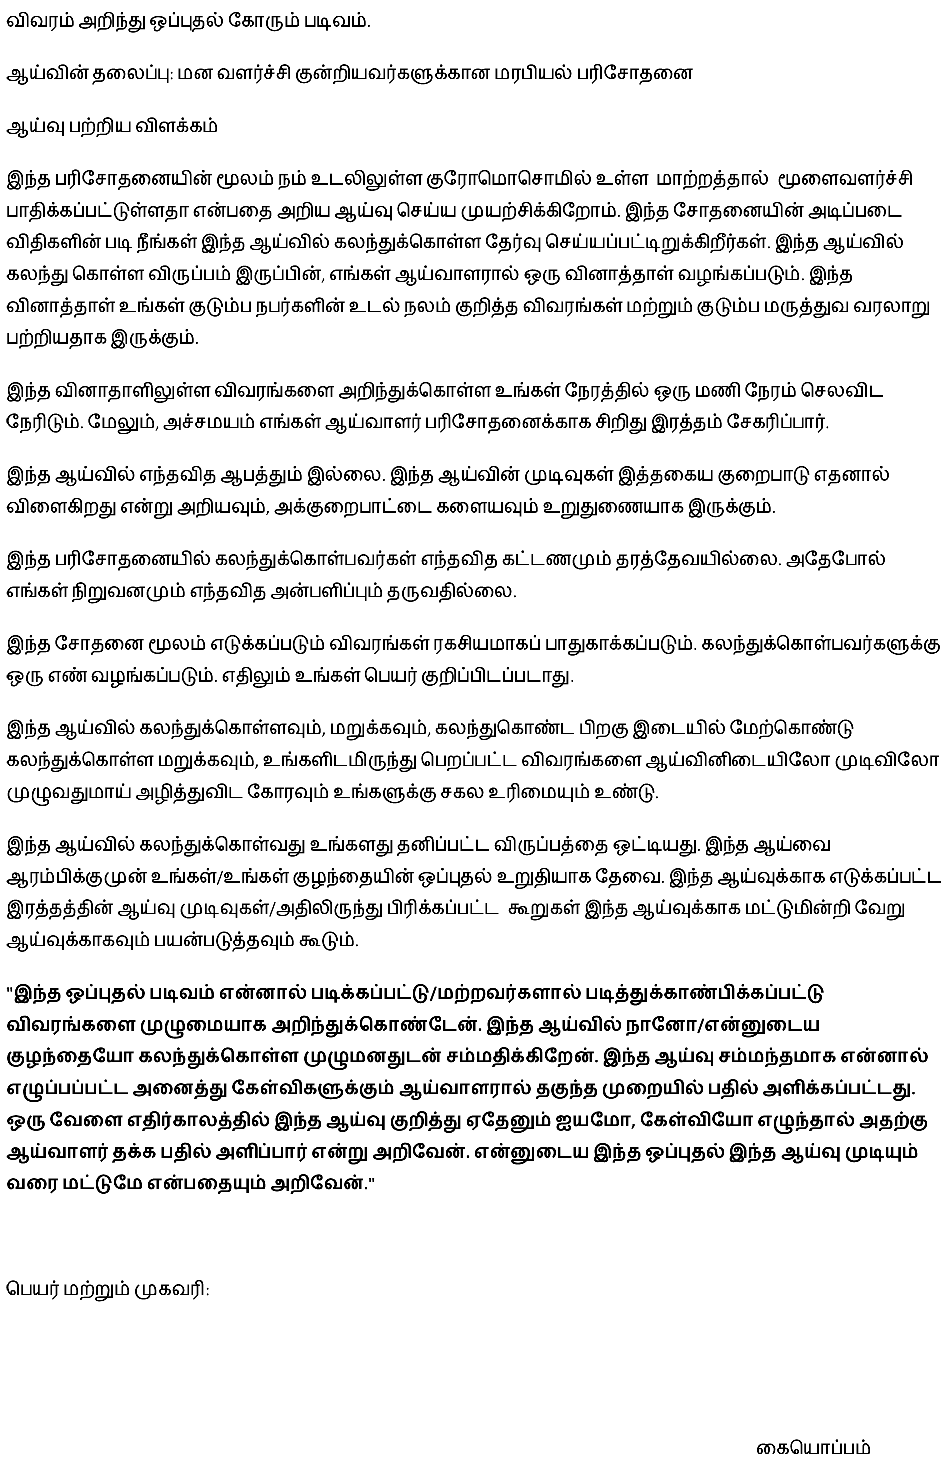
\includegraphics[width=\linewidth,height=\textheight,keepaspectratio]{Appendices/Appendix3c.pdf}}
\end{minipage}

\chapter*{test black}

\color{black}
\textbf{Shruthi Mohan}, Teena Koshy, Solomon FD Paul, Latha Ravichandran,
Venkatachalam P. Detection of subtelomeric rearrangements in \textit{idiopathic
  mental retardation} by \textsc{fluorescence in situ hybridization}. 5th Annual
Conference on Genetic and Molecular Diagnosis in Modern Medicine, SRM, Chennai;
2012.

abcdefghijklmnopqrstuvwxyz. ABCDEFGHIJKLMNOPQRSTUVWXYZ. 1234567890.
\textit{abcdefghijklmnopqrstuvwxyz. ABCDEFGHIJKLMNOPQRSTUVWXYZ. 1234567890.}
\textbf{abcdefghijklmnopqrstuvwxyz. ABCDEFGHIJKLMNOPQRSTUVWXYZ. 1234567890.}

\color{CoolBlack}
\textbf{Shruthi Mohan}, Teena Koshy, Solomon FD Paul, Latha Ravichandran,
Venkatachalam P. Detection of subtelomeric rearrangements in \textit{idiopathic
  mental retardation} by \textsc{fluorescence in situ hybridization}. 5th Annual
Conference on Genetic and Molecular Diagnosis in Modern Medicine, SRM, Chennai;
2012.

abcdefghijklmnopqrstuvwxyz. ABCDEFGHIJKLMNOPQRSTUVWXYZ. 1234567890.
\textit{abcdefghijklmnopqrstuvwxyz. ABCDEFGHIJKLMNOPQRSTUVWXYZ. 1234567890.}
\textbf{abcdefghijklmnopqrstuvwxyz. ABCDEFGHIJKLMNOPQRSTUVWXYZ. 1234567890.}

\color{richblack}
\textbf{Shruthi Mohan}, Teena Koshy, Solomon FD Paul, Latha Ravichandran,
Venkatachalam P. Detection of subtelomeric rearrangements in \textit{idiopathic
  mental retardation} by \textsc{fluorescence in situ hybridization}. 5th Annual
Conference on Genetic and Molecular Diagnosis in Modern Medicine, SRM, Chennai;
2012.

abcdefghijklmnopqrstuvwxyz. ABCDEFGHIJKLMNOPQRSTUVWXYZ. 1234567890.
\textit{abcdefghijklmnopqrstuvwxyz. ABCDEFGHIJKLMNOPQRSTUVWXYZ. 1234567890.}
\textbf{abcdefghijklmnopqrstuvwxyz. ABCDEFGHIJKLMNOPQRSTUVWXYZ. 1234567890.}

